% Created by tikzDevice version 0.12.6 on 2025-04-07 02:49:46
% !TEX encoding = UTF-8 Unicode
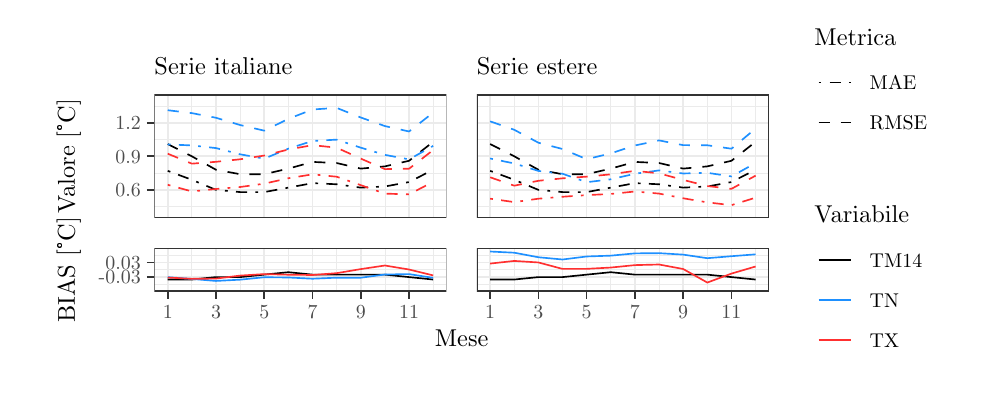
\begin{tikzpicture}[x=1pt,y=1pt]
\definecolor{fillColor}{RGB}{255,255,255}
\path[use as bounding box,fill=fillColor] (0,0) rectangle (341.43,128.04);
\begin{scope}
\path[clip] (  0.00,  0.00) rectangle (341.43,128.04);
\definecolor{drawColor}{RGB}{255,255,255}

\path[draw=drawColor,line width= 0.6pt,line join=round,line cap=round,fill=fillColor] (  0.00,  0.00) rectangle (341.43,128.04);
\end{scope}
\begin{scope}
\path[clip] (  5.50, 53.84) rectangle (156.82,122.54);
\definecolor{drawColor}{RGB}{255,255,255}
\definecolor{fillColor}{RGB}{255,255,255}

\path[draw=drawColor,line width= 0.6pt,line join=round,line cap=round,fill=fillColor] (  5.50, 53.84) rectangle (156.82,122.54);
\end{scope}
\begin{scope}
\path[clip] (156.82, 53.84) rectangle (335.93,122.54);
\definecolor{drawColor}{RGB}{255,255,255}
\definecolor{fillColor}{RGB}{255,255,255}

\path[draw=drawColor,line width= 0.6pt,line join=round,line cap=round,fill=fillColor] (156.82, 53.84) rectangle (335.93,122.54);
\end{scope}
\begin{scope}
\path[clip] (  5.50,  5.50) rectangle (156.82, 53.84);
\definecolor{drawColor}{RGB}{255,255,255}
\definecolor{fillColor}{RGB}{255,255,255}

\path[draw=drawColor,line width= 0.6pt,line join=round,line cap=round,fill=fillColor] (  5.50,  5.50) rectangle (156.82, 53.84);
\end{scope}
\begin{scope}
\path[clip] (156.82,  5.50) rectangle (335.93, 53.84);
\definecolor{drawColor}{RGB}{255,255,255}
\definecolor{fillColor}{RGB}{255,255,255}

\path[draw=drawColor,line width= 0.6pt,line join=round,line cap=round,fill=fillColor] (156.82,  5.50) rectangle (335.93, 53.84);
\end{scope}
\begin{scope}
\path[clip] ( 45.82, 59.34) rectangle (151.32,103.76);
\definecolor{fillColor}{RGB}{255,255,255}

\path[fill=fillColor] ( 45.82, 59.34) rectangle (151.32,103.76);
\definecolor{drawColor}{gray}{0.92}

\path[draw=drawColor,line width= 0.3pt,line join=round] ( 45.82, 63.38) --
	(151.32, 63.38);

\path[draw=drawColor,line width= 0.3pt,line join=round] ( 45.82, 75.49) --
	(151.32, 75.49);

\path[draw=drawColor,line width= 0.3pt,line join=round] ( 45.82, 87.61) --
	(151.32, 87.61);

\path[draw=drawColor,line width= 0.3pt,line join=round] ( 45.82, 99.73) --
	(151.32, 99.73);

\path[draw=drawColor,line width= 0.3pt,line join=round] ( 59.33, 59.34) --
	( 59.33,103.76);

\path[draw=drawColor,line width= 0.3pt,line join=round] ( 76.77, 59.34) --
	( 76.77,103.76);

\path[draw=drawColor,line width= 0.3pt,line join=round] ( 94.21, 59.34) --
	( 94.21,103.76);

\path[draw=drawColor,line width= 0.3pt,line join=round] (111.65, 59.34) --
	(111.65,103.76);

\path[draw=drawColor,line width= 0.3pt,line join=round] (129.09, 59.34) --
	(129.09,103.76);

\path[draw=drawColor,line width= 0.3pt,line join=round] (146.52, 59.34) --
	(146.52,103.76);

\path[draw=drawColor,line width= 0.6pt,line join=round] ( 45.82, 69.43) --
	(151.32, 69.43);

\path[draw=drawColor,line width= 0.6pt,line join=round] ( 45.82, 81.55) --
	(151.32, 81.55);

\path[draw=drawColor,line width= 0.6pt,line join=round] ( 45.82, 93.67) --
	(151.32, 93.67);

\path[draw=drawColor,line width= 0.6pt,line join=round] ( 50.61, 59.34) --
	( 50.61,103.76);

\path[draw=drawColor,line width= 0.6pt,line join=round] ( 68.05, 59.34) --
	( 68.05,103.76);

\path[draw=drawColor,line width= 0.6pt,line join=round] ( 85.49, 59.34) --
	( 85.49,103.76);

\path[draw=drawColor,line width= 0.6pt,line join=round] (102.93, 59.34) --
	(102.93,103.76);

\path[draw=drawColor,line width= 0.6pt,line join=round] (120.37, 59.34) --
	(120.37,103.76);

\path[draw=drawColor,line width= 0.6pt,line join=round] (137.81, 59.34) --
	(137.81,103.76);
\definecolor{drawColor}{RGB}{0,0,0}

\path[draw=drawColor,line width= 0.6pt,dash pattern=on 1pt off 3pt on 4pt off 3pt ,line join=round] ( 50.61, 76.30) --
	( 59.33, 73.07) --
	( 68.05, 69.43) --
	( 76.77, 68.63) --
	( 85.49, 68.63) --
	( 94.21, 70.24) --
	(102.93, 71.86) --
	(111.65, 71.45) --
	(120.37, 70.24) --
	(129.09, 70.65) --
	(137.81, 72.26) --
	(146.52, 76.70);

\path[draw=drawColor,line width= 0.6pt,dash pattern=on 4pt off 4pt ,line join=round] ( 50.61, 85.99) --
	( 59.33, 81.55) --
	( 68.05, 76.70) --
	( 76.77, 75.09) --
	( 85.49, 75.09) --
	( 94.21, 77.11) --
	(102.93, 79.53) --
	(111.65, 79.13) --
	(120.37, 77.11) --
	(129.09, 77.92) --
	(137.81, 79.94) --
	(146.52, 86.80);
\definecolor{drawColor}{RGB}{30,144,255}

\path[draw=drawColor,line width= 0.6pt,dash pattern=on 1pt off 3pt on 4pt off 3pt ,line join=round] ( 50.61, 85.86) --
	( 59.33, 85.49) --
	( 68.05, 84.53) --
	( 76.77, 82.28) --
	( 85.49, 80.71) --
	( 94.21, 84.33) --
	(102.93, 87.10) --
	(111.65, 87.58) --
	(120.37, 84.68) --
	(129.09, 82.08) --
	(137.81, 80.44) --
	(146.52, 85.31);

\path[draw=drawColor,line width= 0.6pt,dash pattern=on 4pt off 4pt ,line join=round] ( 50.61, 98.21) --
	( 59.33, 97.16) --
	( 68.05, 95.48) --
	( 76.77, 92.86) --
	( 85.49, 90.82) --
	( 94.21, 95.09) --
	(102.93, 98.48) --
	(111.65, 99.05) --
	(120.37, 95.58) --
	(129.09, 92.48) --
	(137.81, 90.53) --
	(146.52, 97.33);
\definecolor{drawColor}{RGB}{255,48,48}

\path[draw=drawColor,line width= 0.6pt,dash pattern=on 1pt off 3pt on 4pt off 3pt ,line join=round] ( 50.61, 71.27) --
	( 59.33, 68.86) --
	( 68.05, 69.75) --
	( 76.77, 70.46) --
	( 85.49, 71.67) --
	( 94.21, 73.63) --
	(102.93, 75.04) --
	(111.65, 74.18) --
	(120.37, 71.13) --
	(129.09, 68.07) --
	(137.81, 67.81) --
	(146.52, 72.34);

\path[draw=drawColor,line width= 0.6pt,dash pattern=on 4pt off 4pt ,line join=round] ( 50.61, 82.50) --
	( 59.33, 78.90) --
	( 68.05, 79.57) --
	( 76.77, 80.48) --
	( 85.49, 81.83) --
	( 94.21, 84.02) --
	(102.93, 85.58) --
	(111.65, 84.68) --
	(120.37, 80.72) --
	(129.09, 76.93) --
	(137.81, 77.07) --
	(146.52, 83.82);
\definecolor{drawColor}{gray}{0.20}

\path[draw=drawColor,line width= 0.6pt,line join=round,line cap=round] ( 45.82, 59.34) rectangle (151.32,103.76);
\end{scope}
\begin{scope}
\path[clip] (  0.00,  0.00) rectangle (341.43,128.04);
\definecolor{drawColor}{gray}{0.30}

\node[text=drawColor,anchor=base east,inner sep=0pt, outer sep=0pt, scale=  0.72] at ( 40.87, 66.97) {0.6};

\node[text=drawColor,anchor=base east,inner sep=0pt, outer sep=0pt, scale=  0.72] at ( 40.87, 79.09) {0.9};

\node[text=drawColor,anchor=base east,inner sep=0pt, outer sep=0pt, scale=  0.72] at ( 40.87, 91.20) {1.2};
\end{scope}
\begin{scope}
\path[clip] (  0.00,  0.00) rectangle (341.43,128.04);
\definecolor{drawColor}{gray}{0.20}

\path[draw=drawColor,line width= 0.6pt,line join=round] ( 43.07, 69.43) --
	( 45.82, 69.43);

\path[draw=drawColor,line width= 0.6pt,line join=round] ( 43.07, 81.55) --
	( 45.82, 81.55);

\path[draw=drawColor,line width= 0.6pt,line join=round] ( 43.07, 93.67) --
	( 45.82, 93.67);
\end{scope}
\begin{scope}
\path[clip] (  0.00,  0.00) rectangle (341.43,128.04);
\definecolor{drawColor}{RGB}{0,0,0}

\node[text=drawColor,rotate= 90.00,anchor=base,inner sep=0pt, outer sep=0pt, scale=  0.88] at ( 17.06, 81.55) {Valore [\textdegree C]};
\end{scope}
\begin{scope}
\path[clip] (  0.00,  0.00) rectangle (341.43,128.04);
\definecolor{drawColor}{RGB}{0,0,0}

\node[text=drawColor,anchor=base west,inner sep=0pt, outer sep=0pt, scale=  0.88] at ( 45.82,110.98) {Serie italiane};
\end{scope}
\begin{scope}
\path[clip] (162.32, 59.34) rectangle (267.82,103.76);
\definecolor{fillColor}{RGB}{255,255,255}

\path[fill=fillColor] (162.32, 59.34) rectangle (267.82,103.76);
\definecolor{drawColor}{gray}{0.92}

\path[draw=drawColor,line width= 0.3pt,line join=round] (162.32, 63.38) --
	(267.82, 63.38);

\path[draw=drawColor,line width= 0.3pt,line join=round] (162.32, 75.49) --
	(267.82, 75.49);

\path[draw=drawColor,line width= 0.3pt,line join=round] (162.32, 87.61) --
	(267.82, 87.61);

\path[draw=drawColor,line width= 0.3pt,line join=round] (162.32, 99.73) --
	(267.82, 99.73);

\path[draw=drawColor,line width= 0.3pt,line join=round] (175.84, 59.34) --
	(175.84,103.76);

\path[draw=drawColor,line width= 0.3pt,line join=round] (193.27, 59.34) --
	(193.27,103.76);

\path[draw=drawColor,line width= 0.3pt,line join=round] (210.71, 59.34) --
	(210.71,103.76);

\path[draw=drawColor,line width= 0.3pt,line join=round] (228.15, 59.34) --
	(228.15,103.76);

\path[draw=drawColor,line width= 0.3pt,line join=round] (245.59, 59.34) --
	(245.59,103.76);

\path[draw=drawColor,line width= 0.3pt,line join=round] (263.03, 59.34) --
	(263.03,103.76);

\path[draw=drawColor,line width= 0.6pt,line join=round] (162.32, 69.43) --
	(267.82, 69.43);

\path[draw=drawColor,line width= 0.6pt,line join=round] (162.32, 81.55) --
	(267.82, 81.55);

\path[draw=drawColor,line width= 0.6pt,line join=round] (162.32, 93.67) --
	(267.82, 93.67);

\path[draw=drawColor,line width= 0.6pt,line join=round] (167.12, 59.34) --
	(167.12,103.76);

\path[draw=drawColor,line width= 0.6pt,line join=round] (184.55, 59.34) --
	(184.55,103.76);

\path[draw=drawColor,line width= 0.6pt,line join=round] (201.99, 59.34) --
	(201.99,103.76);

\path[draw=drawColor,line width= 0.6pt,line join=round] (219.43, 59.34) --
	(219.43,103.76);

\path[draw=drawColor,line width= 0.6pt,line join=round] (236.87, 59.34) --
	(236.87,103.76);

\path[draw=drawColor,line width= 0.6pt,line join=round] (254.31, 59.34) --
	(254.31,103.76);
\definecolor{drawColor}{RGB}{0,0,0}

\path[draw=drawColor,line width= 0.6pt,dash pattern=on 1pt off 3pt on 4pt off 3pt ,line join=round] (167.12, 76.30) --
	(175.84, 73.07) --
	(184.55, 69.43) --
	(193.27, 68.63) --
	(201.99, 68.63) --
	(210.71, 70.24) --
	(219.43, 71.86) --
	(228.15, 71.45) --
	(236.87, 70.24) --
	(245.59, 70.65) --
	(254.31, 72.26) --
	(263.03, 76.70);

\path[draw=drawColor,line width= 0.6pt,dash pattern=on 4pt off 4pt ,line join=round] (167.12, 85.99) --
	(175.84, 81.55) --
	(184.55, 76.70) --
	(193.27, 75.09) --
	(201.99, 75.09) --
	(210.71, 77.11) --
	(219.43, 79.53) --
	(228.15, 79.13) --
	(236.87, 77.11) --
	(245.59, 77.92) --
	(254.31, 79.94) --
	(263.03, 86.80);
\definecolor{drawColor}{RGB}{30,144,255}

\path[draw=drawColor,line width= 0.6pt,dash pattern=on 1pt off 3pt on 4pt off 3pt ,line join=round] (167.12, 80.76) --
	(175.84, 78.97) --
	(184.55, 76.28) --
	(193.27, 75.25) --
	(201.99, 72.20) --
	(210.71, 73.25) --
	(219.43, 75.25) --
	(228.15, 76.47) --
	(236.87, 75.35) --
	(245.59, 75.60) --
	(254.31, 74.28) --
	(263.03, 79.13);

\path[draw=drawColor,line width= 0.6pt,dash pattern=on 4pt off 4pt ,line join=round] (167.12, 94.19) --
	(175.84, 91.13) --
	(184.55, 86.47) --
	(193.27, 84.19) --
	(201.99, 80.50) --
	(210.71, 82.63) --
	(219.43, 85.47) --
	(228.15, 87.30) --
	(236.87, 85.59) --
	(245.59, 85.55) --
	(254.31, 84.30) --
	(263.03, 91.58);
\definecolor{drawColor}{RGB}{255,48,48}

\path[draw=drawColor,line width= 0.6pt,dash pattern=on 1pt off 3pt on 4pt off 3pt ,line join=round] (167.12, 66.25) --
	(175.84, 65.00) --
	(184.55, 66.24) --
	(193.27, 66.94) --
	(201.99, 67.54) --
	(210.71, 67.95) --
	(219.43, 68.84) --
	(228.15, 68.09) --
	(236.87, 66.39) --
	(245.59, 64.91) --
	(254.31, 63.91) --
	(263.03, 66.61);

\path[draw=drawColor,line width= 0.6pt,dash pattern=on 4pt off 4pt ,line join=round] (167.12, 73.97) --
	(175.84, 70.94) --
	(184.55, 72.71) --
	(193.27, 73.60) --
	(201.99, 74.21) --
	(210.71, 75.04) --
	(219.43, 76.32) --
	(228.15, 75.40) --
	(236.87, 73.03) --
	(245.59, 70.81) --
	(254.31, 69.80) --
	(263.03, 74.57);
\definecolor{drawColor}{gray}{0.20}

\path[draw=drawColor,line width= 0.6pt,line join=round,line cap=round] (162.32, 59.34) rectangle (267.82,103.76);
\end{scope}
\begin{scope}
\path[clip] (  0.00,  0.00) rectangle (341.43,128.04);
\definecolor{drawColor}{RGB}{0,0,0}

\node[text=drawColor,anchor=base west,inner sep=0pt, outer sep=0pt, scale=  0.88] at (162.32,110.98) {Serie estere};
\end{scope}
\begin{scope}
\path[clip] ( 45.82, 32.79) rectangle (151.32, 48.34);
\definecolor{fillColor}{RGB}{255,255,255}

\path[fill=fillColor] ( 45.82, 32.79) rectangle (151.32, 48.34);
\definecolor{drawColor}{gray}{0.92}

\path[draw=drawColor,line width= 0.3pt,line join=round] ( 45.82, 35.26) --
	(151.32, 35.26);

\path[draw=drawColor,line width= 0.3pt,line join=round] ( 45.82, 40.56) --
	(151.32, 40.56);

\path[draw=drawColor,line width= 0.3pt,line join=round] ( 45.82, 45.86) --
	(151.32, 45.86);

\path[draw=drawColor,line width= 0.3pt,line join=round] ( 59.33, 32.79) --
	( 59.33, 48.34);

\path[draw=drawColor,line width= 0.3pt,line join=round] ( 76.77, 32.79) --
	( 76.77, 48.34);

\path[draw=drawColor,line width= 0.3pt,line join=round] ( 94.21, 32.79) --
	( 94.21, 48.34);

\path[draw=drawColor,line width= 0.3pt,line join=round] (111.65, 32.79) --
	(111.65, 48.34);

\path[draw=drawColor,line width= 0.3pt,line join=round] (129.09, 32.79) --
	(129.09, 48.34);

\path[draw=drawColor,line width= 0.3pt,line join=round] (146.52, 32.79) --
	(146.52, 48.34);

\path[draw=drawColor,line width= 0.6pt,line join=round] ( 45.82, 37.91) --
	(151.32, 37.91);

\path[draw=drawColor,line width= 0.6pt,line join=round] ( 45.82, 43.21) --
	(151.32, 43.21);

\path[draw=drawColor,line width= 0.6pt,line join=round] ( 50.61, 32.79) --
	( 50.61, 48.34);

\path[draw=drawColor,line width= 0.6pt,line join=round] ( 68.05, 32.79) --
	( 68.05, 48.34);

\path[draw=drawColor,line width= 0.6pt,line join=round] ( 85.49, 32.79) --
	( 85.49, 48.34);

\path[draw=drawColor,line width= 0.6pt,line join=round] (102.93, 32.79) --
	(102.93, 48.34);

\path[draw=drawColor,line width= 0.6pt,line join=round] (120.37, 32.79) --
	(120.37, 48.34);

\path[draw=drawColor,line width= 0.6pt,line join=round] (137.81, 32.79) --
	(137.81, 48.34);
\definecolor{drawColor}{RGB}{0,0,0}

\path[draw=drawColor,line width= 0.6pt,line join=round] ( 50.61, 37.03) --
	( 59.33, 37.03) --
	( 68.05, 37.91) --
	( 76.77, 37.91) --
	( 85.49, 38.80) --
	( 94.21, 39.68) --
	(102.93, 38.80) --
	(111.65, 38.80) --
	(120.37, 38.80) --
	(129.09, 38.80) --
	(137.81, 37.91) --
	(146.52, 37.03);
\definecolor{drawColor}{RGB}{30,144,255}

\path[draw=drawColor,line width= 0.6pt,line join=round] ( 50.61, 37.89) --
	( 59.33, 37.24) --
	( 68.05, 36.52) --
	( 76.77, 36.98) --
	( 85.49, 37.86) --
	( 94.21, 37.77) --
	(102.93, 37.32) --
	(111.65, 37.70) --
	(120.37, 37.69) --
	(129.09, 38.85) --
	(137.81, 38.99) --
	(146.52, 37.64);
\definecolor{drawColor}{RGB}{255,48,48}

\path[draw=drawColor,line width= 0.6pt,line join=round] ( 50.61, 37.75) --
	( 59.33, 37.28) --
	( 68.05, 37.37) --
	( 76.77, 38.45) --
	( 85.49, 39.00) --
	( 94.21, 38.77) --
	(102.93, 38.67) --
	(111.65, 39.33) --
	(120.37, 40.80) --
	(129.09, 42.10) --
	(137.81, 40.65) --
	(146.52, 38.52);
\definecolor{drawColor}{gray}{0.20}

\path[draw=drawColor,line width= 0.6pt,line join=round,line cap=round] ( 45.82, 32.79) rectangle (151.32, 48.34);
\end{scope}
\begin{scope}
\path[clip] (  0.00,  0.00) rectangle (341.43,128.04);
\definecolor{drawColor}{gray}{0.30}

\node[text=drawColor,anchor=base east,inner sep=0pt, outer sep=0pt, scale=  0.72] at ( 40.87, 35.45) {-0.03};

\node[text=drawColor,anchor=base east,inner sep=0pt, outer sep=0pt, scale=  0.72] at ( 40.87, 40.75) {0.03};
\end{scope}
\begin{scope}
\path[clip] (  0.00,  0.00) rectangle (341.43,128.04);
\definecolor{drawColor}{gray}{0.20}

\path[draw=drawColor,line width= 0.6pt,line join=round] ( 43.07, 37.91) --
	( 45.82, 37.91);

\path[draw=drawColor,line width= 0.6pt,line join=round] ( 43.07, 43.21) --
	( 45.82, 43.21);
\end{scope}
\begin{scope}
\path[clip] (  0.00,  0.00) rectangle (341.43,128.04);
\definecolor{drawColor}{gray}{0.20}

\path[draw=drawColor,line width= 0.6pt,line join=round] ( 50.61, 30.04) --
	( 50.61, 32.79);

\path[draw=drawColor,line width= 0.6pt,line join=round] ( 68.05, 30.04) --
	( 68.05, 32.79);

\path[draw=drawColor,line width= 0.6pt,line join=round] ( 85.49, 30.04) --
	( 85.49, 32.79);

\path[draw=drawColor,line width= 0.6pt,line join=round] (102.93, 30.04) --
	(102.93, 32.79);

\path[draw=drawColor,line width= 0.6pt,line join=round] (120.37, 30.04) --
	(120.37, 32.79);

\path[draw=drawColor,line width= 0.6pt,line join=round] (137.81, 30.04) --
	(137.81, 32.79);
\end{scope}
\begin{scope}
\path[clip] (  0.00,  0.00) rectangle (341.43,128.04);
\definecolor{drawColor}{gray}{0.30}

\node[text=drawColor,anchor=base,inner sep=0pt, outer sep=0pt, scale=  0.72] at ( 50.61, 22.91) {1};

\node[text=drawColor,anchor=base,inner sep=0pt, outer sep=0pt, scale=  0.72] at ( 68.05, 22.91) {3};

\node[text=drawColor,anchor=base,inner sep=0pt, outer sep=0pt, scale=  0.72] at ( 85.49, 22.91) {5};

\node[text=drawColor,anchor=base,inner sep=0pt, outer sep=0pt, scale=  0.72] at (102.93, 22.91) {7};

\node[text=drawColor,anchor=base,inner sep=0pt, outer sep=0pt, scale=  0.72] at (120.37, 22.91) {9};

\node[text=drawColor,anchor=base,inner sep=0pt, outer sep=0pt, scale=  0.72] at (137.81, 22.91) {11};
\end{scope}
\begin{scope}
\path[clip] (  0.00,  0.00) rectangle (341.43,128.04);
\definecolor{drawColor}{RGB}{0,0,0}

\node[text=drawColor,rotate= 90.00,anchor=base,inner sep=0pt, outer sep=0pt, scale=  0.88] at ( 17.06, 40.56) {BIAS [\textdegree C]};
\end{scope}
\begin{scope}
\path[clip] (162.32, 32.79) rectangle (267.82, 48.34);
\definecolor{fillColor}{RGB}{255,255,255}

\path[fill=fillColor] (162.32, 32.79) rectangle (267.82, 48.34);
\definecolor{drawColor}{gray}{0.92}

\path[draw=drawColor,line width= 0.3pt,line join=round] (162.32, 35.26) --
	(267.82, 35.26);

\path[draw=drawColor,line width= 0.3pt,line join=round] (162.32, 40.56) --
	(267.82, 40.56);

\path[draw=drawColor,line width= 0.3pt,line join=round] (162.32, 45.86) --
	(267.82, 45.86);

\path[draw=drawColor,line width= 0.3pt,line join=round] (175.84, 32.79) --
	(175.84, 48.34);

\path[draw=drawColor,line width= 0.3pt,line join=round] (193.27, 32.79) --
	(193.27, 48.34);

\path[draw=drawColor,line width= 0.3pt,line join=round] (210.71, 32.79) --
	(210.71, 48.34);

\path[draw=drawColor,line width= 0.3pt,line join=round] (228.15, 32.79) --
	(228.15, 48.34);

\path[draw=drawColor,line width= 0.3pt,line join=round] (245.59, 32.79) --
	(245.59, 48.34);

\path[draw=drawColor,line width= 0.3pt,line join=round] (263.03, 32.79) --
	(263.03, 48.34);

\path[draw=drawColor,line width= 0.6pt,line join=round] (162.32, 37.91) --
	(267.82, 37.91);

\path[draw=drawColor,line width= 0.6pt,line join=round] (162.32, 43.21) --
	(267.82, 43.21);

\path[draw=drawColor,line width= 0.6pt,line join=round] (167.12, 32.79) --
	(167.12, 48.34);

\path[draw=drawColor,line width= 0.6pt,line join=round] (184.55, 32.79) --
	(184.55, 48.34);

\path[draw=drawColor,line width= 0.6pt,line join=round] (201.99, 32.79) --
	(201.99, 48.34);

\path[draw=drawColor,line width= 0.6pt,line join=round] (219.43, 32.79) --
	(219.43, 48.34);

\path[draw=drawColor,line width= 0.6pt,line join=round] (236.87, 32.79) --
	(236.87, 48.34);

\path[draw=drawColor,line width= 0.6pt,line join=round] (254.31, 32.79) --
	(254.31, 48.34);
\definecolor{drawColor}{RGB}{0,0,0}

\path[draw=drawColor,line width= 0.6pt,line join=round] (167.12, 37.03) --
	(175.84, 37.03) --
	(184.55, 37.91) --
	(193.27, 37.91) --
	(201.99, 38.80) --
	(210.71, 39.68) --
	(219.43, 38.80) --
	(228.15, 38.80) --
	(236.87, 38.80) --
	(245.59, 38.80) --
	(254.31, 37.91) --
	(263.03, 37.03);
\definecolor{drawColor}{RGB}{30,144,255}

\path[draw=drawColor,line width= 0.6pt,line join=round] (167.12, 47.15) --
	(175.84, 46.72) --
	(184.55, 45.08) --
	(193.27, 44.27) --
	(201.99, 45.36) --
	(210.71, 45.66) --
	(219.43, 46.48) --
	(228.15, 46.56) --
	(236.87, 46.03) --
	(245.59, 44.74) --
	(254.31, 45.46) --
	(263.03, 46.13);
\definecolor{drawColor}{RGB}{255,48,48}

\path[draw=drawColor,line width= 0.6pt,line join=round] (167.12, 42.80) --
	(175.84, 43.75) --
	(184.55, 43.20) --
	(193.27, 40.87) --
	(201.99, 40.89) --
	(210.71, 41.36) --
	(219.43, 42.24) --
	(228.15, 42.46) --
	(236.87, 40.83) --
	(245.59, 35.94) --
	(254.31, 39.18) --
	(263.03, 41.74);
\definecolor{drawColor}{gray}{0.20}

\path[draw=drawColor,line width= 0.6pt,line join=round,line cap=round] (162.32, 32.79) rectangle (267.82, 48.34);
\end{scope}
\begin{scope}
\path[clip] (  0.00,  0.00) rectangle (341.43,128.04);
\definecolor{drawColor}{gray}{0.20}

\path[draw=drawColor,line width= 0.6pt,line join=round] (167.12, 30.04) --
	(167.12, 32.79);

\path[draw=drawColor,line width= 0.6pt,line join=round] (184.55, 30.04) --
	(184.55, 32.79);

\path[draw=drawColor,line width= 0.6pt,line join=round] (201.99, 30.04) --
	(201.99, 32.79);

\path[draw=drawColor,line width= 0.6pt,line join=round] (219.43, 30.04) --
	(219.43, 32.79);

\path[draw=drawColor,line width= 0.6pt,line join=round] (236.87, 30.04) --
	(236.87, 32.79);

\path[draw=drawColor,line width= 0.6pt,line join=round] (254.31, 30.04) --
	(254.31, 32.79);
\end{scope}
\begin{scope}
\path[clip] (  0.00,  0.00) rectangle (341.43,128.04);
\definecolor{drawColor}{gray}{0.30}

\node[text=drawColor,anchor=base,inner sep=0pt, outer sep=0pt, scale=  0.72] at (167.12, 22.91) {1};

\node[text=drawColor,anchor=base,inner sep=0pt, outer sep=0pt, scale=  0.72] at (184.55, 22.91) {3};

\node[text=drawColor,anchor=base,inner sep=0pt, outer sep=0pt, scale=  0.72] at (201.99, 22.91) {5};

\node[text=drawColor,anchor=base,inner sep=0pt, outer sep=0pt, scale=  0.72] at (219.43, 22.91) {7};

\node[text=drawColor,anchor=base,inner sep=0pt, outer sep=0pt, scale=  0.72] at (236.87, 22.91) {9};

\node[text=drawColor,anchor=base,inner sep=0pt, outer sep=0pt, scale=  0.72] at (254.31, 22.91) {11};
\end{scope}
\begin{scope}
\path[clip] (  0.00,  0.00) rectangle (341.43,128.04);
\definecolor{drawColor}{RGB}{0,0,0}

\node[text=drawColor,anchor=base,inner sep=0pt, outer sep=0pt, scale=  0.88] at (156.82, 12.71) {Mese};
\end{scope}
\begin{scope}
\path[clip] (  0.00,  0.00) rectangle (341.43,128.04);
\definecolor{fillColor}{RGB}{255,255,255}

\path[fill=fillColor] (278.82, 81.00) rectangle (330.43,134.18);
\end{scope}
\begin{scope}
\path[clip] (  0.00,  0.00) rectangle (341.43,128.04);
\definecolor{drawColor}{RGB}{0,0,0}

\node[text=drawColor,anchor=base west,inner sep=0pt, outer sep=0pt, scale=  0.88] at (284.32,121.77) {Metrica};
\end{scope}
\begin{scope}
\path[clip] (  0.00,  0.00) rectangle (341.43,128.04);
\definecolor{fillColor}{RGB}{255,255,255}

\path[fill=fillColor] (284.32,100.96) rectangle (298.78,115.41);
\end{scope}
\begin{scope}
\path[clip] (  0.00,  0.00) rectangle (341.43,128.04);
\definecolor{drawColor}{RGB}{0,0,0}

\path[draw=drawColor,line width= 0.6pt,dash pattern=on 1pt off 3pt on 4pt off 3pt ,line join=round] (285.77,108.18) -- (297.33,108.18);
\end{scope}
\begin{scope}
\path[clip] (  0.00,  0.00) rectangle (341.43,128.04);
\definecolor{fillColor}{RGB}{255,255,255}

\path[fill=fillColor] (284.32, 86.50) rectangle (298.78,100.96);
\end{scope}
\begin{scope}
\path[clip] (  0.00,  0.00) rectangle (341.43,128.04);
\definecolor{drawColor}{RGB}{0,0,0}

\path[draw=drawColor,line width= 0.6pt,dash pattern=on 4pt off 4pt ,line join=round] (285.77, 93.73) -- (297.33, 93.73);
\end{scope}
\begin{scope}
\path[clip] (  0.00,  0.00) rectangle (341.43,128.04);
\definecolor{drawColor}{RGB}{0,0,0}

\node[text=drawColor,anchor=base west,inner sep=0pt, outer sep=0pt, scale=  0.72] at (304.28,105.72) {MAE};
\end{scope}
\begin{scope}
\path[clip] (  0.00,  0.00) rectangle (341.43,128.04);
\definecolor{drawColor}{RGB}{0,0,0}

\node[text=drawColor,anchor=base west,inner sep=0pt, outer sep=0pt, scale=  0.72] at (304.28, 91.27) {RMSE};
\end{scope}
\begin{scope}
\path[clip] (  0.00,  0.00) rectangle (341.43,128.04);
\definecolor{fillColor}{RGB}{255,255,255}

\path[fill=fillColor] (278.82,  2.37) rectangle (328.65, 70.00);
\end{scope}
\begin{scope}
\path[clip] (  0.00,  0.00) rectangle (341.43,128.04);
\definecolor{drawColor}{RGB}{0,0,0}

\node[text=drawColor,anchor=base west,inner sep=0pt, outer sep=0pt, scale=  0.88] at (284.32, 57.59) {Variabile};
\end{scope}
\begin{scope}
\path[clip] (  0.00,  0.00) rectangle (341.43,128.04);
\definecolor{fillColor}{RGB}{255,255,255}

\path[fill=fillColor] (284.32, 36.78) rectangle (298.78, 51.23);
\end{scope}
\begin{scope}
\path[clip] (  0.00,  0.00) rectangle (341.43,128.04);
\definecolor{drawColor}{RGB}{0,0,0}

\path[draw=drawColor,line width= 0.6pt,line join=round] (285.77, 44.00) -- (297.33, 44.00);
\end{scope}
\begin{scope}
\path[clip] (  0.00,  0.00) rectangle (341.43,128.04);
\definecolor{fillColor}{RGB}{255,255,255}

\path[fill=fillColor] (284.32, 22.32) rectangle (298.78, 36.78);
\end{scope}
\begin{scope}
\path[clip] (  0.00,  0.00) rectangle (341.43,128.04);
\definecolor{drawColor}{RGB}{30,144,255}

\path[draw=drawColor,line width= 0.6pt,line join=round] (285.77, 29.55) -- (297.33, 29.55);
\end{scope}
\begin{scope}
\path[clip] (  0.00,  0.00) rectangle (341.43,128.04);
\definecolor{fillColor}{RGB}{255,255,255}

\path[fill=fillColor] (284.32,  7.87) rectangle (298.78, 22.32);
\end{scope}
\begin{scope}
\path[clip] (  0.00,  0.00) rectangle (341.43,128.04);
\definecolor{drawColor}{RGB}{255,48,48}

\path[draw=drawColor,line width= 0.6pt,line join=round] (285.77, 15.10) -- (297.33, 15.10);
\end{scope}
\begin{scope}
\path[clip] (  0.00,  0.00) rectangle (341.43,128.04);
\definecolor{drawColor}{RGB}{0,0,0}

\node[text=drawColor,anchor=base west,inner sep=0pt, outer sep=0pt, scale=  0.72] at (304.28, 41.54) {TM14};
\end{scope}
\begin{scope}
\path[clip] (  0.00,  0.00) rectangle (341.43,128.04);
\definecolor{drawColor}{RGB}{0,0,0}

\node[text=drawColor,anchor=base west,inner sep=0pt, outer sep=0pt, scale=  0.72] at (304.28, 27.09) {TN};
\end{scope}
\begin{scope}
\path[clip] (  0.00,  0.00) rectangle (341.43,128.04);
\definecolor{drawColor}{RGB}{0,0,0}

\node[text=drawColor,anchor=base west,inner sep=0pt, outer sep=0pt, scale=  0.72] at (304.28, 12.63) {TX};
\end{scope}
\end{tikzpicture}
